\section{Linear Programming}

\subsection{Problem}
A factory produces tables and chairs
\begin{itemize}
	\item 1 table requires 1 unit of metal and 3 units of wood
	\item 1 chair requires 2 units of metal and 1 unit of wood
	\item The factory has 600 units (900 units) of metal (wood)
	\item The profit of 1 table is 100\EUR and 1 chair is 100\EUR
\end{itemize}
\paragraph{Question} How many tables/chairs to produce to maximize the profit?
$$x_1: \#tables \; to \; produce \Rightarrow x_1 \geq 0$$
$$x_2: \#chairs \; to \; produce \Rightarrow x_2 \geq 0$$
\paragraph{Profit} $100(x_1+x_2) = 100 x_1 + 100 x_2$
\paragraph{Constraints} $x_1 + 2x_2 \leq 600$ and $3x_1+x_2 \leq 900$
\paragraph{Maximize}  \textcolor{green}{$100x_1+100x_2$} 
\paragraph{Subject to (s.t.)} \textcolor{yellow}{$x_1 + 2x_2 \leq 600$} and \textcolor{orange}{$3x_1+x_2 \leq 900$} and \textcolor{blue}{$x_1,x_2 \geq 0$} \\
\begin{center}
	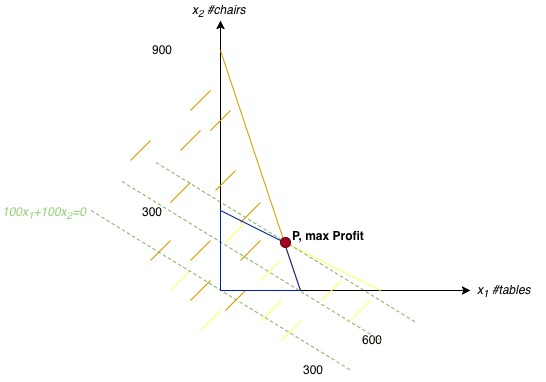
\includegraphics[scale=0.75]{img/dia1}
\end{center}
$$100x_1+100x_2 = 30000 (x_1=0,x_2 = 300 \equiv x_1 = 900, x_2=0)$$
\paragraph{Observation} As the line $100x_1+100x_2=c$ moves toward $P$, the profit gets increased. $\Rightarrow$ $P$ is optimal (intersection of $\stackrel{(1)}{x_1}+2x_2=600$, $3x_1+\stackrel{(2)}{x_2} = 900$) \\
\begin{itemize}
	\item[(1)] $\Rightarrow x_1 = 600 - 2x_2$
	\item[(2)] \begin{align*} &\stackrel{(1)}{=}2(600-2x_2)+x_2 = 900 \\
	& 1800 - 6x_2+x_1 = 900 \\
	&5x_2 = 900 \Rightarrow x_2 = 180
	& \Rightarrow x_1 = 240
	\end{align*}
\end{itemize}
\paragraph{Optimal} $x_1 = 240, x_2 = 180$
\paragraph{Profit} 42000 \EUR
\paragraph{Different cases}
\begin{center}
	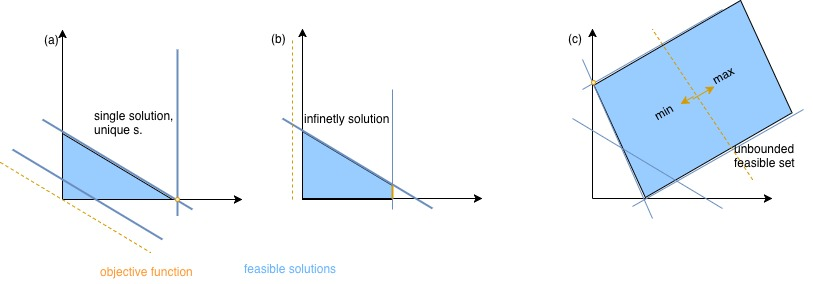
\includegraphics[scale=0.5]{img/dia3}
\end{center}
(a),(b) $\Rightarrow$ bounded feasible solution $\Rightarrow \exists$ solution $\Rightarrow$ corner solution \\
(c) $\Rightarrow$ feasible (corner solution) or infeasible/unbounded
$$\text{(a),(b),(c)} \exists solution \Rightarrow \exists corner solution$$
\begin{itemize}
	\item[(1)] bounded feasible (a),(b)
	\item[(2)] unbounded feasible (c) min
	\item[(3)] unbounded infeasible (c) max
	\item[NOT] \sout{un}bounded infeasible
\end{itemize}

\subsubsection{Generalization}
\paragraph{Maximize} $c_1x_1 + c_2x_2 + ... + c_nx_n \rightarrow$ objective function (linear)
\paragraph{Minimize} \phantom, 
\paragraph{Subject to} constraints set \\
\begin{center}
\begin{tabular}{c|c|c}
	& one-of & \\
	$a_{11}x_1+a_{12}x_2+...a_{1n}x_n$ &  & $b_1$ \\ 
	& $\leq$ & \\
	$a_{21}x_1+a_{22}x_2+...a_{2n}x_n$ & & $b_2$ \\
	& $=$ & \\
	... & & ... \\
	& $\geq$ & \\
	$a_{m1}x_1+a_{m2}x_2+...a_{mn}x_n$ & & $b_m$ \\
\end{tabular}
\end{center}
optional non-negativity constraint: $(x_1,x_2,...,x_n \geq 0)$ 

\subsection{Another example: Max-flow}
\paragraph{Input} directed graph $G=(V,E),s,t \in V$ \\
$indegree(s) = outdegree(t) = 0$ \\
capacities $c: E \rightarrow \mathbb{R}^+$
\paragraph{Output} find $f: E \rightarrow \mathbb{R}^+$ such that:
\begin{itemize}
	\item[(1)] $\forall(u,v) \in E: 0 \leq f(u,v) \leq c(u,v)$
	\item[(2)] $\sum_{(u,v) \in E}f(u.v) = \sum_{(v,u) \in E}f(u,v) \forall u \in V-{s,t}$
	\item[(3)] $max \sum_{(s,v) \in E}f(s,v)$
\end{itemize}
\subsubsection{LP formulation}
maximize $\sum_{(s,v) \in E}f(s,v)$ (3) \\
s.t.
\paragraph{Constraints} $f(u,v) \leq c(u,v) \forall (u,v) \in E (\approx 1)$ \\
$\sum_{(u,v) \in E}f(u.v) = \sum_{(v,u) \in E}f(u,v) \forall u \in V-{s,t}$ (2)
\paragraph{Negativity} $f(u,v) \geq 0 \forall (u,v) \in E$ 

\subsubsection{Geometric representation in higher dimensions}
\begin{center}
	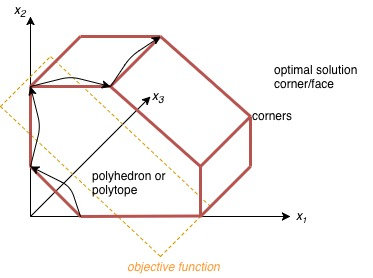
\includegraphics[scale=0.5]{img/dia2}
\end{center}
Simplex: Move from corner to corner
\subsection{Standard form}
\paragraph{Maximization} $c_1x_1 + c_2x_2 + ... + c_nx_n$
\paragraph{Subject to} \begin{align*}
	a_{11}x_1 + a_{12}x_2  + ... + a_{1n}x_n  &\leq b_1 \\
	a_{21}x_1 + a_{22}x_2  + ... + a_{2n}x_n  &\leq b_2 \\
	... \\
	a_{m1}x_1 + a_{m2}x_2  + ... + a_{mn}x_n  &\leq b_m \\
	x_1,x_2,...,x_n  &^\geq 0 \\
\end{align*}
\paragraph{Maximization} $C^Tx$
\paragraph{Subject to} \begin{align*}
	Ax &\leq b \\
	x & \geq 0
\end{align*}
$$C = \begin{bmatrix}
c_1 \\ c_2 \\ ... \\ c_n
\end{bmatrix} \Rightarrow C^T = \begin{bmatrix}
c_1,...,c_n
\end{bmatrix}$$
$$x_1 = \begin{bmatrix}
x_1 \\ x_2 \\ ... \\ x_n
\end{bmatrix} \hspace*{1cm} b = \begin{bmatrix}
b_1 \\ ... \\ b_m
\end{bmatrix} \hspace{1cm} A = \begin{bmatrix}
a_{11} & a_{12} & ... & a_{1n} \\
a_{21} & a_{22} & ... & a_{2n} \\
... \\
a_{m1} & a_{m2} & ... & a_{mn} 
\end{bmatrix}$$
First step of (pre-processing) simplex to bring the input LP to the standard form.

Why not in standard form?
\begin{itemize}
\item[(1)] minimize $c_1x_1+c_2x_2+...+c_nx_n \Leftrightarrow$ maximize $-c_1x_1-c_2x_2-...-c_nx_n$
\item[(2)] Equality $a_{j1}x_1 + a_{j2}x_2 + ... + a_{jn}x_n = b_j$ \\ $\Leftrightarrow a_{j1}x_1 + a_{j2}x_2 + ... + a_{jn}x_n \leq b_j$ \\
$\& (-) a_{j1}x_1 +(-) a_{j2}x_2 +(-) ... +(-) a_{jn}x_n \geq (\leq) b_j$
\item[(3)] $\geq$ inequality $a_{j1}x_1 + a_{j2}x_2 + ... + a_{jn}x_n \geq b_j \Leftrightarrow -a_{j1}x_1 - a_{j2}x_2 - ... - a_{jn}x_n \leq b_j$
\item[(4)] Absence of non-negativity constraints.
\end{itemize}
Replace: \\ 
$x_j \rightarrow x_j' \& x_j''$ \\
$x_j = x_j'-x_j'';x_j',x_j'' \geq 0$
\paragraph{Example} ~ \\
\begin{tabular}{ccccc}
minimize& $-2x_1+3x_2$ && maximize &$2x_1-3x_2'+3x_2''$ \\
s.t. & \textcolor{red}{$x_1+x_2 = 7$} && s.t. & $x_1+x_2'-x_2'' \leq 7$ \\
& $x_1-2x_2 \leq 5$ & $\rightarrow$ && $-x_1-x_2'+x_2'' \leq -7$ \\
& $x_1 \geq 0$ &&& $x_1-2x_2''+2x_2'' \leq 5$ \\
&&&& $x_1,x_2',x_2'' \geq 0$ \\
\end{tabular} \\
\textcolor{red}{non-negativity for $x_1=x_2'-x_2''$}

\subsection{The simplex method}

\subsubsection{By an example}
\begin{align*}
\text{maximize} & 5x_1+4x_2+3x_3 \\
\text{s.t.} & 2x_1+3x_2+x_3 \leq 5 \\
\text{(in standard} & 4x_1 + x_2 + 2x_3 \leq 11 \\
\text{form)} & 3x_1 + 4x_1 + 2x_3 \leq 8 \\
& x_1,x_2,x_3 \geq 0
\end{align*}
\begin{itemize}
\item[(1)] Introduce a name for the objective function 
$$J = 5x_1+4x_2+3x_3$$
\item[(2)] Introduce a slack (difference between right and left) variable for each constraint
$$x_4 = 5-2x_1-3x_2-x_3 ; x_4 \geq 0$$
$$\text{right-left side $\geq 0 \Rightarrow$ right-left side $=x_4, x_4 \geq 0$}$$
\end{itemize}
Standardform $\rightarrow$ slack form
\begin{align*}
\text{maximize} J &= \textcolor{orange}{5x_1 + 4x_2 + 3x_3} \\
\textcolor{green}{x_4} &= 5-\textcolor{orange}{2x_1-3x_2-x_3} (1) \\ 
\textcolor{green}{x_5} &= 11-\textcolor{orange}{4x_1-x_2-2x_3}  (2) \\
\textcolor{green}{x_6} &= 8-\textcolor{orange}{3x_1-4x_2-2x_3}  (3) \\
x_1,x_2,x_3,x_4,x_5,x_6 \geq 0
\end{align*}
\textcolor{green}{non-zero variables}, \textcolor{orange}{zero variables}
\paragraph{Idea} Start with a solution $(x_1,x_2,x_3,x_4,x_5,x_6)$, dinf another solution $(\overline{x_1},\overline{x_2},\overline{x_3},\overline{x_4},\overline{x_5},\overline{x_6})$ s.t, iterate $5x_1+4x_2+3x_2 \leq 5\overline{x_1} + 4\overline{x_2} + 3\overline{x_3}$
\paragraph{Problem} Initial feasible solution to start the iteration? \\
In the example: Easy! $x_1=x_2=x_3=0.x_4=5,x_5=11,x_6=8,J=0$
\paragraph{Assumption} $b_1,b_2,...,b_n \geq 0 \Rightarrow x_1 = x_2 = ... = x_n = 0$ is feasible \\
How can we find a better solution than $J=0$?
\paragraph{Observation} If we increase $x_1$ (or $x_2$ od $x_3$) (positive coefficient), then $J$ will also increas, but we must ensure that $x_4,x_5,x_6 \geq 0$ \\
Since $x_2=x_3 = 0$
\begin{itemize}
	\item $x_4 \geq 0 \Rightarrow 5-2x_1 \geq 0 \Leftrightarrow x_1 \leq \frac{5}{2} 2.5$
	\item $x_5 \geq 0 \Rightarrow 11-4x_1 \geq 0 \Leftrightarrow x_1 \leq \frac{11}{4} = 2.75$ 
	\item $x_6 \geq 0 \Rightarrow 8 -3x_1 \geq 0 \Leftrightarrow x_1 \leq \frac{8}{3}= 2.66...$
\end{itemize}
New solution: $x_1 = \frac{5}{2}, x_2,x_3 = 0, x_4 = 0, x_5 = 1, x_6 = \frac{1}{2} J = \frac{25}{2} = 12.5$ \\
How do we proceed? 
\paragraph{Observation} THe first step was easy beacuse all non-zero variables were expected as linear combination of zero variables ($x_1$ now got non zero).
\begin{itemize}
	\item (1) $\Leftrightarrow 2x_1 = 5-3x_2 -x_3-x_4 \Leftrightarrow x_1 = \frac{5}{2} - \frac{3}{2}x_2 - \frac{1}{3}x_3 - \frac{1}{2}x_4$
	\item $J=5(\frac{5}{2} - \frac{3}{2}x_2 - \frac{1}{3}x_3 - \frac{1}{2}x_4) + 4x_2 + 3x_3 \Leftrightarrow J = \frac{25}{2} - \frac{7}{2}x_2 + \frac{1}{2}x_3 - \frac{5}{2}x_4$
	\item $x_5 = 11 - 4 (\frac{5}{2} - \frac{3}{2}x_2 - \frac{1}{3}x_3 - \frac{1}{2}x_4) - x_2 - 2x_3 \Leftrightarrow x_5 = 1 + 5x_2 + 2x_4$
	\item $x_6 = 8-3(\frac{5}{2} - \frac{3}{2}x_2 - \frac{1}{3}x_3 - \frac{1}{2}x_4) - 4x_2 - 2x_3 \Leftrightarrow x_6 = \frac{1}{2} + \frac{1}{2}x_2 - \frac{1}{2}x_3 + \frac{3}{2}x_4$
\end{itemize}
maximize $J = \frac{25}{2} - \frac{7}{2}x_2 + \frac{1}{2}x_3 - \frac{5}{2}x_4$
\begin{align*}
x_1 &= \frac{5}{2} - \frac{3}{2}x_2 - \frac{1}{3}x_3 - \frac{1}{2}x_4 \\
x_5 &= 1 + 5x_2 + 2x_4 \\
(*)x_6 &= \frac{1}{2} + \frac{1}{2}x_2 - \frac{1}{2}x_3 + \frac{3}{2}x_4 \\
&x_1,...,x_6 \geq 0. x_1,x_5,x_6 \text{ non zero variables}
\end{align*}
\paragraph{Observation} If we increase $x_2$ or $x_4$, then $J$ will decrease (bad idea), so we have to increase $x_3$ (positive coefficient) \\
Since $x_2=x_4 = 0$: \\
\begin{itemize}
	\item $x_1 \geq 0 \Leftrightarrow \frac{5}{2}-\frac{1}{2}x_3 \geq 0 \Leftrightarrow x_3 \leq 5$
	\item $x_5$ does not relate $x_3 \Rightarrow$ not constrained
	\item $x_6 \geq 0 \Leftrightarrow \frac{1}{2}x_3 \geq 0 \Leftrightarrow x_3 \leq 1$
\end{itemize}
New soluion: $x_1 = 2, x_2 = 0, x_3 = 1, x_4 = 0, x_5 = 1, x_6 = 0$ \\
maximize $J = 13 - 3x_2 - x_4 - x_6$ \\
\begin{align*}
\text{s.t. } x_3 &= 1 + x_2 + 3x_4 - 2x_6 (*) \\
x_1 &= 2 - 2x_2 - 2x_4 + x_6 \\
x_5 &= 1 + 5x_2 + 2x_4 \\
&x_1,x_2,...,x_6 \geq 0
\end{align*}
If $x_2,x_4,x_6$ are increased, then $J$ decreases $\Rightarrow J$ is optimal. 
\begin{enumerate}
	\item The last system is equivalent to the first
	\item In the last system all variables must be non-zero (cant't decrease variable to $<0$ e.g. $13-3\cdot(-2) \lightning x_2 \geq 0$!)
\end{enumerate}	

\subsubsection{Theory}
\begin{itemize}
	\item Preprocessing step: general LP $\stackrel{rules}{\rightarrow}$ LP in standard form. 
	\item Assumption
	\begin{enumerate}
		\item maximize $c_1x_1+c_2x_2+...+c_nx_n$ \\
		s.t. $a_{j1}x_1+a_{j2}x_2+...a_{jn}x_n \leq bj \forall j=1,2,...,m$ \\
		$x_i \geq 0 \forall i = 1,2,...,n$
		\item $b_1,...,b_m \geq 0 \Rightarrow x_1=x_2=...=x_n=0$ is feasible.
	\end{enumerate} 
\end{itemize}
Transform to Slack Form: \\
maximize $J = \sum_{i=1}^nc_1x_i$ (Initial Dictionary)\\
s.t. $x_{n+1} = b_j - \sum_{i=1}^na_{ji}x_i \forall j = 1,...,m$ \\
$x_1 \geq 0 \forall i = 1,...,n+m$ \\
$x_{n+1}$ are slcak variables. \\
zero-value variables ($x_1 \forall i = 1,...,n$)$\rightarrow$ non-basic.\\
non-zero-value variables ($x_i \forall i = n+1,...,n+m$) $\rightarrow$ basic. \\
At every step of the simplex
\begin{itemize}
	\item one basic variable becomes non-basic
	\item one non-basic variable becomes basic
\end{itemize}
At some step of the simplex: \\
$B$: the set of indices of the basic variables \\
$N$: the set of indices of the non-basic variables \\
maximize $J = \underbrace{\overline{J}}_{\text{value of obj. funciton}} + \sum_{i \in N}\overline{c}_ix_i$ \\
s.t. $x_i = \overline{b}_i - \sum_{j \in N}\overline{a_{ij}}x_j \forall i \in B$ \\
$x_i \geq 0 \forall i \in B \cup N$ 
\paragraph{Entering variable}  Is one in $N^+ = \{x_i, \overline{c_i}>0 i \in N\}$ (if $x_i$ is increased, then $J$ is increased)
\begin{itemize}
	\item $N^+ = \emptyset \Rightarrow J = \overline{J}$ is optimal (since increasing any of the non-basic variables will decrease $J$)
	\item $|N^+| > 1$: select the entering variable as the one with the smalles index. 
	\item[$\Rightarrow$] let $x_k$ be the entering variable.
\end{itemize}
\paragraph{Exiting variable} We have to ensure that all basic variables $x_i \geq 0 \forall i \in B \stackrel{\forall i \in N  -\{k\} x_i = 0}{\Longrightarrow}$ \\
$$\Leftrightarrow \overline{b_i} - \sum_{j \in N}\overline{a_{ij}}x_j \geq 0 \forall i \in B$$ 
$$\Leftrightarrow \overline{b_i} - \overline{a_{ik}}x_k \geq 0 \forall i \in B$$ 
$$\stackrel{a_{ik}>0 \lor a_{ik}<0}{\Longleftrightarrow} \begin{cases}
x_k \leq \frac{\overline{b_i}}{\overline{a_{ik}}} & a_{ik} > 0 \\
x_k \geq \frac{\overline{b_i}}{\overline{a_{ik}}} & a_{ik} < 0\\
\end{cases}$$
We chose the exiting variable as the one for which $\frac{\overline{b_i}}{a_{ik}}$ is minimum and $a_{ik} > 0$ \\
\fbox{\parbox{\linewidth}{Note: If $\overline{a_{ik}}<0$, there is no restriction on how much we can increase $x_k \Rightarrow$ the System is unboundes and $J \rightarrow + \infty$}} 

\subsection{Duality}
Each LP (original/primal LP) has an associated, called dual, LP.
\paragraph{Origninal LP (standard form)} $n$ variables, $m$ constraints \\
\begin{align*}
\text{maximize } & c_1x_1+c_2x_2+...+c_nx_n \\
\text{s.t. } &a_{11}x_x+a_{12}x_2+...+a_{1n}x_n \leq b_1 \\
&... \\
&a_{m1}x_1+a_{m2}x_2+...+a_{mn}x_n \leq b_m \\
&x_1,...,x_n \geq 0
\end{align*}
\paragraph{Dual LP (standard minimal form)} $m$ variables, $n$ constraints \\
\begin{align*}
\text{minimize } & b_1y_1+b_2y_2+...+b_my_m \\
\text{s.t. } &a_{11}y_x+a_{21}y_2+...+a_{m1}y_m \geq c_1 \\
&... \\
&a_{1n}y_1+a_{2n}y_2+...+a_{mn}y_m \geq c_n\\
&y_1,...,y_m \geq 0
\end{align*}
\paragraph{Primal} ~ \\
\begin{align*}
\text{maximize } &c^Tx \\
\text{s.t. } & Ax \leq b \\
& x \geq 0
\end{align*}
$$c = \begin{bmatrix}
c_1 \\ c_2 \\ ... \\ c_n
\end{bmatrix} \Rightarrow C^T = \begin{bmatrix}
c_1,...,c_n
\end{bmatrix}$$
$$x = \begin{bmatrix}
x_1 \\ x_2 \\ ... \\ x_n
\end{bmatrix} \hspace*{1cm} b = \begin{bmatrix}
b_1 \\ ... \\ b_m
\end{bmatrix} \hspace{1cm} A = \begin{bmatrix}
a_{11} & a_{12} & ... & a_{1n} \\
a_{21} & a_{22} & ... & a_{2n} \\
... \\
a_{m1} & a_{m2} & ... & a_{mn}
\end{bmatrix} \hspace*{1cm} y = \begin{bmatrix}
y_1 \\ y_2 \\ ... \\ y_m
\end{bmatrix}
$$
\paragraph{Dual} ~ \\
\begin{align*}
\text{minimize } &c^Tx \\
\text{s.t. } & yA \geq c^T \\
& y \geq 0
\end{align*}
\begin{center}
\begin{tabular}{c|cccc|c}
& $x_1$ & $x_2$ & ... & $x_n$ & \\ \hline 
$y_1$ & $a_{11}$ & $a_{12}$ & ... & $a_{1n}$ & $\leq b_1$ \\
$y_2$ & $a_{21}$ & $a_{22}$ & ... & $a_{2n}$ & $\leq b_2$ \\
... & ... & ... &...& ...& ... \\
$y_n$ & $a_{m1}$ & $a_{m2}$ & ... & $a_{mn}$ & $\leq b_m$ \\ \hline 
& $\geq c_1$ & $\geq c_2$ & ... & $\geq c_n$ & \\
\end{tabular} 
\end{center}
1. equation of dual: $y$ columns and the $x_1$ column. \\
1. equation of orimal: $x$ row and $y_1$ row
\begin{align*}
\text{maximize } &100x_1 + 100x_2 \\
\text{s.t. } &x_1+2x_2 \leq 600 \\
&3x_1+x_2 \leq 900 \\
x_1,x_2 \geq 0
\end{align*}
Dual:
\begin{align*}
\text{minimize } &600y_1+900y_2 \\
\text{s.t. } &y_1+3y_2 \geq 100 \\
&2y_1+y_2\geq 100 \\
y_1,y_2 \geq 0 
\end{align*}

\subsubsection{Weak duality theorem}
If $x = [x_1,...,x_n]^T$ is a feasible solution of the primal \\
and $y = [y_1,...,y_n]^T$ is a feasible solution of the dual \\
$\Rightarrow c^T \leq y^Tb$ \\
Any feasible solution of the primal is upper bounded by any feasible solution of the dual.
\paragraph{Proof} $x$ is feasible in the primal $\Rightarrow Ax \leq b; x \geq 0 \stackrel{ (y^T*)\geq 0}{\Rightarrow} \textcolor{red}{y^TAx} \leq y^Tb$ \\
$y$ is feasible in the dual $\Rightarrow yA \geq c; y \geq 0 \stackrel{\cdot (*x) \geq 0}{\Rightarrow} \textcolor{red}{y^TAx} \geq c^Tx$ 
$$\Rightarrow c^Tx \leq y^TAx \leq y^Tb	$$
$$\underbrace{-------------op}_{primal \; values}---------\underbrace{od-------------}_{dual \; values}$$
op = optimal primal value, od = optimal dual value \\
Is there a Gap between op and od? $\stackrel{Strong \; duality \; theorem}{\longrightarrow}$ $\nexists$ Gap

\paragraph{Corollary} If $x,y$ are feasible for the primal and the dual s.t. $c^Tx = y^Tb$, then $x\&y$ are optimal.